%\documentclass{svjour3}                     % onecolumn (standard format)
%\documentclass[smallcondensed]{svjour3}     % onecolumn (ditto)
\documentclass[smallextended]{svjour3}       % onecolumn (second format)
%\documentclass[twocolumn]{svjour3}          % twocolumn
%
\smartqed  % flush right qed marks, e.g. at end of proof
%
\usepackage{adjustbox}
\RequirePackage{fix-cm}
\usepackage{graphicx}
\usepackage{wrapfig}
%

\journalname{Empirical Software Engineering}
%
\usepackage{color,colortbl}
\usepackage{xcolor}
\begin{document}

\title{On the Sociology of Reuse} %\thanks{Grants or other notes
%about the article that should go on the front page should be
%placed here. General acknowledgments should be placed at the end of the article.}
\subtitle{Fostering Effective Artifact Sharing for SE Research}

%\titlerunning{Short form of title}        % if too long for running head

\author{Maria  Baldassarre     
\and Ben  Hermann \and
        Tim Menzies %etc.
}

%\authorrunning{Short form of author list} % if too long for running head

\institute{baldassarre.teresa@gmail.com
\at
              first address \\
              Tel.: +123-45-678910\\
              Fax: +123-45-678910\\
              \email{fauthor@example.com}           %  \\
%             \emph{Present address:} of F. Author  %  if needed
           \and
         ben.hermann@cs.tu-dortmund.de \at
         }
         


\date{Received: date / Accepted: date}
% The correct dates will be entered by the editor

\newcommand{\bi}{\begin{itemize}}
\newcommand{\ei}{\end{itemize}}
\maketitle

\begin{abstract}
%insert blah blah here 
There are many ways the SE community could collect and organize its collective knowledge. 
This paper describes a large space of options in designing artifact evaluation panels, as well as criteria for selecting what kind of artifact evaluation panel is right for a particular conferences.
% Based on their experience with numerous 
% code-sharing and data -sharing initiatives in SE,
% the authors argue sociological , not technological, issues are the major indicator for successful community curation  of ideas (code or data). With appropriate (and easy to design) community reward structures, a thriving joint collective of people and their ideas can be be created.  
\keywords{First keyword \and Second keyword \and More}
% \PACS{PACS code1 \and PACS code2 \and more}
% \subclass{MSC code1 \and MSC code2 \and more}
\end{abstract}

\section{Introduction}
\label{intro}

Peer-reviewed publications are the most visible and highly regarded product of research. 
In the process leading to this publication many other artifacts are created. 
In the past decade the software engineering community has given an increased attention to these research artifacts and is subjecting them to their own peer-review process called \emph{artifact evaluation}. 
A recent study~\cite{10.1145/3368089.3409767} found that the goals of this process have not yet solidified and are still being discussed. 
In this paper we wish to contribute a new perspective to this discussion highlighting the sociology and tradition of reuse in the software engineering community, 

To this end, we describe the conflicting interests in the current practice of artifact evaluation, extending on the findings by Hermann et al. 
In our observations we also draw from our own experience in sharing and reusing research artifact since 2005~\cite{menzies2013guest}. 
We also argue that:
\begin{quote}
{\bf
the artifact types, currently considered in artifact evaluation are only a fraction of those actually created by researchers in the field of software engineering\cite{chambers2019s}.}
\end{quote}

While artifact evaluation most certainly elevated the availability and prestige of research artifact, we believe its greatest potential benefit is in fostering a culture of sharing and reuse in software engineering.

We advocate for several procedural changes, especially in the role of the reviewer, to leverage this benefit.
Artifact evaluation currently is organized analogously to paper review.
This applies particularly to the role of the reviewer whose task is to assess the possible repeatability of the experiments conducted through or with the artifact.

Reviewers can take either the role of a judge, demanding the adherence to strict rules and standards based on the submitted version, or the role of a shepherd, strengthening the artifact through close communication with the authors. 
The first role includes insisting on a perfect artifact at the time of submission without a chance for authors to correct win or transgressions. 
Unlike in papers, small mistakes can have catastrophic consequences for artifacts rendering them unusable. 
Mistyping a character may leave out an important processing step in an experiment. 
The artifact will then go unrecognized as currently it has to be evaluated at the same venue as the paper.
 
%There is much recent interest in {\em artifact evaluation panels} at software engineering and programming language conferences. In the last five year we have seen the mean number of papers offering artifacts   grow from XXX to YYY (at the ASE, ICSE, FSE, EMSE conferences~\cite{benxxx}).
%Between us, the authors of this paper have served on the review panel on nine different artifact committees for major SE conferences. One of us   organized the first SE artifacts evaluation panels (for FSE'2011). Another of us has serving data artifacts to the SE research community since 2005~\cite{menzies2013guest}. Based on that experience, we offer the following suggestions about artifact evaluations.

Moreover, in recent years the evaluation category of \emph{reusability} was added as an additional distinction evaluating artifacts created with more care towards a possible reuse. 
However, there is no current process in place assessing if artifact are in fact reused. 

%Much  of that the current artifact evaluation effort is focused on assessing the supposed reusability of new code-based artifacts. However:
%\begin{itemize}
%\item 
%Very little of the current work checks if  artifacts   actually get reused. 
%\item
%Very little of the current work checks non-code-based artifacts. For a list of non-code-based artifacts, see Table~\ref{types}.
%\end{itemize}

In the following, we note that artifact panel organizers are free to change these trend, if they want to. 
To help with that, this paper describes a large space of options in designing artifact evaluation panels, as well as criteria for selecting what kind of artifact evaluation panel is right for a particular conferences.


\begin{table}[!t]
\caption{Artifact types from SE publications. Current artifact evaluation committees in software engineering and programming conferences typically review just the green items 19,20,21,22,23.
Also, usually, items 1,2,3,4,5,6,7,8,9 are typically  evaluated in 
registered reports venues \cite{chambers2019s} from qualitative researchers (who are getting their experimental protocols checked before they start their experiments).
That said, there is nothing in principle stopping artifact review committees from 
reviewing any of the following. For example, the IEEE Requirements Engineering Conference 2019 ran a artifacts track that reviewed items from both ends of this list.}\label{types}
{\scriptsize
\begin{tabular}{|p{.96\linewidth}|}\hline
\rowcolor{gray!15}\begin{enumerate}
\item
Motivational statements or reports or challenge statements or lists of open issues that prompt an analysis;
\item Hypotheses, about expected effects in some area;
\item Checklists used to design the analysis (see also   Checklist Manifesto http://atulgawande.com/book/the-checklist-manifesto/);
\item Bibliographies, comprehensive, annotated, and insightful (e.g. showing the development or open areas in a field);
\item Study instruments such as surveys interview scripts, etc;
\item Statistical tests used to analyze results (along with some notes explaining why or when this test is necessary);
\item Commentary on scripts used in the analysis;
\item Examples of particularly informative visualizations (e.g. see Sparklines
http://tiny.cc/sparklines)
\item Baseline results against which new work can be compared;
\end{enumerate}
\\\hline
\begin{enumerate}
 \setcounter{enumi}{11}
\item Sampling procedures e.g. ``how did you choose the projects you studied?'';
\item Patterns describing best practices for performing this kind of analysis;
\item Anti-patterns describing cautionary tales of ``gotchas'' to avoid when doing this kind of work;
\item Negative results that are anti-patterns, backed up by empirical results;
\item Tutorial materials: Guides to help newcomers become proficient in the area. Some of these tutorial materials may be generated by the researcher and others may be collected from other sources.
\item New results that offer guidance on how to best handle future problems.
\item Future work: From the results, there many be speculations about open issues of future issues that might become the motivation for the next round of research.
The actual text of an author's papers;
\end{enumerate}\\\hline

\rowcolor{green!5}\begin{enumerate}
 \setcounter{enumi}{18}
 
\item Any data used in an analysis
\begin{itemize}
\item
Either raw from a project;
\item
Or, if that is too large, some smaller derived product. Note that some data is too large to fit into the standard on-line freely available repos (e.g. Github only allows 1GB reps). For such data, we suggest using some other on-line storage; e.g. Zenodo accepts  50GB files and  higher quotas can be requested and granted on a case-by-case basis.
\end{itemize}
\item Scripts used to perform the analysis (the main analysis or the subsequent statistical tests or visualizations; e.g. the Python Sparklines generator). Scripts can also implement some of the patterns identified by the paper.
\item Executable models that can generate exemplar data; or which offer an executable form of current hypotheses;
\item Programs that realize the algorithms presented or used in the paper;
\item Delivery tools to let novices automatically rerun the analysis; e.g.
\begin{itemize}
\item
  Config management files that can
  \begin{itemize}
\item
build the system/ paper from raw material and/or
\item
update the relevant files using some package manager
\end{itemize}
\item
Virtual machines containing all the above scripts, data, etc, pre-configured such that a newcomer can automatically run the old analysis.
\end{itemize}
\end{enumerate}\\\hline
\end{tabular}}
\end{table}

\clearpage
\section{Motivating Artifact Sharing and Reuse in SE}
Artifacts broadly support the goals of open science \cite{Mendez2020}. Decades of research into the scientific process shows that sharing artifacts from Table \ref{types} has many benefits, including individual motivation like improved citations to broader impact such as industry transfer and increased collaboration in the community. For example, the PROMISE repository \cite{Sayyad2005} has led to XXX. 

Artifacts are also essential to building a culture of replication and reproducibility, already acknowledged as important in SE \cite{2020arXiv201102861S}. Fields such as psychology have had many early results thrown into doubt because of a failure to replicate the original findings~\cite{Schimmack2020}. Sharing research protocols and data allows for other research teams to conduct severe tests of our original studies, strengthening (or rejecting) these initial findings. In medicine, drug companies are required by law to share the research protocols and outcomes of their drug trials, something that has become of vital recent importance (albeit not without challenges \cite{DeVito2020}). In physics and astronomy, artifact sharing is so commonplace that large community infrastructure exist solely to ensure data sharing, not least because governments which fund these costly experiments insist on it. Indeed, a founding impetus for the World Wide Web was the need for the EU's high energy physics network, CERN, to facilitate knowledge sharing~\cite{tbl90}\footnote{And Tim Berners-Lee himself has said ``Had the technology been proprietary, and in my total control, it would probably not have taken off.'' Another argument for artifacts!}.

Managing the replication and artifact sharing process is important. In psychology ill-feeling on the part of those whose initial findings have not replicated is rife. There is a perception that replication is done poorly, that failed replications are desirable, and that the role of exploratory research is disregarded \cite{Schimmack2020}. In our own experience we have seen reviewers exhausted by the additional burden of reviewing (and compiling, debugging, evaluating) artifacts. Thus we argue it is important to understand the sociological factors behind reuse and artifact sharing to maintain a healthy community. We provide suggestions below.

% The discreditation trap 
% The social media trap
% Gaps from here to there
% 0. A: goal is not reusable, but the goal is community
% 0b Border list of artifacts
% 1.Before “Is this a good idea step?”
% 2Do: artifact Need tools for interaction.  Hotcrp (communciation++)  cant do double blind right now (after paper acceptance)
% 3After: contribute.md 
% from Googel but see below

\section{Reviewing Practices for Artifact Committees}

\begin{wrapfigure}{r}{2in}
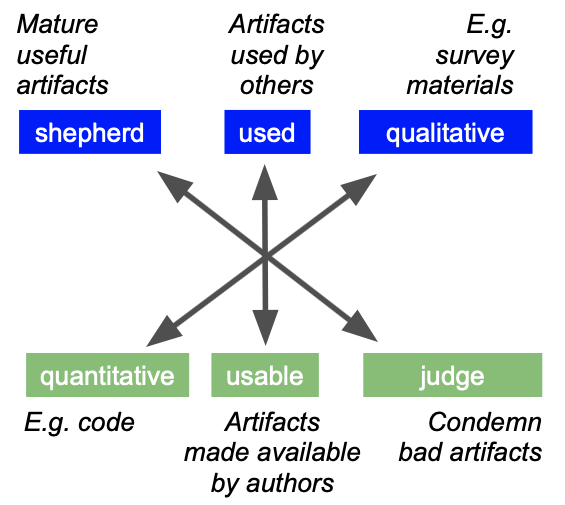
\includegraphics[width=2in]{dimensions.png}
\caption{Current
artifact evaluation processes focuses mostly on judging if quantitative artifacts are ready to be used.
Next generation artifact evaluation processes should also ensure they recognize artifacts that have been used (by other researchers) and which cover the spectrum of both quantitative and qualitative artifacts. There is also a role for artifact evaluation committees to shepherd and mature weaker artifacts.}\label{dims}\end{wrapfigure} 

Before designing an artifact evaluation panel, it is recommended to document that panel's stance on the issues raised in Figure~\ref{dims}. For reasons of exposition, we list these three dimensions with differing ends at each end. In practice, panels can decide to mix and match anywhere they like across these dimensions.
\begin{itemize}
\item ``Judges'' impose strict standards on the artifacts and tend to reject more submissions. ``Shepherds'', on the other hand are more lenient and work with authors to (e.g.) fix one letter typos that stop installation scripts running.
\item ``Qualitataive'' panels typically certify artifacts not related to execution; e.g. see artifacts 1,..,9 in Table~\ref{types}. 
``Quantitative'' panels, on the other hand, only certify artifacts comprising code products
(see items 19,..,24 in Table~\ref{types}). 
\item
Finally, when panels just review artifacts from one conference, they typically
can not determine if an artifact's analysis has been replicated or reproduced (R\&R).
But with  the appropriate changes to their call for submissions, those panels can also check for R\&R.
\end{itemize}



**Rose Festivals and R&R

In the past couple years, during conferences, community activities have been effective but often focused more on “technical” solutions such as giving guidelines for how to do replication packages etc. Community activities such as ROSE as well as “strongly recommending” people to submit open data/materials/code (to be eligible for best paper awards, for example) is more important than more “technical” solutions. The overall “solution” is likely to need to involve multiple activities and decisions on many different levels. 

-- illustrate the idea of rose and how artifact sharing especially focused on levels of 


\section{Tips and Tricks (just at text dump. no structure yet}


TIP1: do not  judge your artifacts committee now by how many functional, reusable, available badges your score. that is just intermediaries. the REAL  goal is replicate and reproduced because that says that we are actually using tht stuff

SUGGESTION1:  as Silvia and Daniel did, have a different process for (functional, reusable, available) and (replicate and reproduced ) . for replicated and reproduced, throw open the gates and allow submissions  any prior SE research work (published at your conference  or elsewhere)  

TIP2: augment your artifacts track with a rose festival in the main technical track. they are great! see http://tiny.cc/rose8. want help organising that? just say the word! 

TIP3: do some work to make replicated and reproduced work. if you dont get many submissions, assign some of your review committee the task of walking thru the proceedings looking for stuff that is based on older stuff. and solicit replicated and reproduced reports from there. 

SUGGESTION2:  Silvia and Daniel: just a suggestion but you could make it mandatory that  submitters AND reviewers specify their home operating systems.  try to match up the home operating system of the artifact with the reviewer (so dont ask mac people to handle artifacts from windows). i know that detail should not matter in this age of docker, but trust me,.. it can save you some time.

TIP4: use github. FYI: ase 21 is using githing. one reason to use github is that it supports multiple  several rounds of very short very controlled interactions between reviewer and author (to e.g. fix one letter typos in the install scripts).  with version control! .  and not to disagree with Silvia and Daneiel but github can support the  qualitative  community. see artifacts RE'19. very successful. we got qual and quant stuff (survey materials on the one hand and natural language parsers for requirements docs on the other hand). the volume at RE'19 was low so i did a lot of nurse maiding (e.g. send me the zip files, i set it up for you on github. look you can make comments. isn't this fun?)

TIP4a: if looking for alternates to github, assess them by how well they support multiple rounds of dialog authors+ reviwer. for example, :  we looked into using hotcrp for artifacts it has a "rounds" system for extended discussions. but as near as we can tell, reviewers have to be different in each round so thumbs down there. 

QUESTION2:   Silvia and Daniel: how are you doing your interaction and queries between authors and reviewers?

TIP4b, for Github, make each submission gets one and only one issue and all activity is addits to the comments in that issue. FSE'20 did a zoo of issues per artifact and it got messy. 

TIP4c: for Gtihub for each reviewer needs an anonymous github id. make sure youvve collected all those BEFORE the review process starts otherwise you can waste a week just on that detail

TIP5: RELAX! with one occasional exception ( assessing functional), eval is usually easy++.  the experience is that most artifacts get badged so we dont need to be crazy strict about this stuff. 

TIP5a:   RELAXing  about assessing "replicated" and "reproduced" 1-2 pages to read, maybe flip over a pdf, and you are  done.  two special cases to watch for: 
(a)  the artifacts committee can run the code so the authors are claiming "replicated!" i don't buy that.  the goal is to get the broader community using the artifacts, not some in-house specialists. 
(b) replications/reproductions at some indusrial site. thats all well and good but there has to be some  **deetails record** of  the work and not just 3 lines saying "and our industrial partners used it. they liked." that does not fly for me

TIP5b:  RELAX about  assessing "available".   takes 20  seconds. is there a DOI badge (which can be got from zenodo in 10 seonds) ? are the artifacts stored in some long term facility (i.e. not the authors home site but, say, zenodo).? then YES it is available. it not, then get back to the author and nudge them into DOIs and maybe zenodo. easy as pie

TIP5c: RELAX about   assessing reusable. think of it as  just "gold star functional". so it the code is ok functional  then thats good. but it if it is GREAT functional then give it a gold star. i.e. call it reusable!

TIP6:  don't under estimate reviewing time.  four badges are fast to review see above but there are some definitely some LONG TAILS when working on "functional". even with docker!

TIP6a:  don't don't don't don't  under staff your eval committee. expect 50 to  70\% of your papers will produce  artifacts.   silvia and daniel understand that-- look at their HUGE committee. in my view,  

TIP6b: dont dont dont overload your reviewers. ideally 2-3 artifacts per reviewer. no more. 


\bibliographystyle{spmpsci}      % basic style, author-year citations
\bibliography{refs}
\end{document}
% end of file template.tex


Before reviewing our current methods, we first take a step back to imaging how our interactions might occur. We do this since, with that higher-level picture in mind, we can better assess our current work. 

Our goal is not replication nor reproduction per se, but all the scientific  interactions  that happen after scientists and engineers share their results and methods. Specifically, we view science as a community that carefully curates a set of ideas, where everyone does each other the courtesy of critiquing and improving everyone else’s ideas.

Nor is our goal artifact “evaluation” per se but artifact evolution. Most researchers do not have the resources of (say) Microsoft to produce elegant turn-key packages that anyone can download and use straight out of the box. Rather, our tools need to be evolved, refactored, improved via community feedback. Clumsy report generation or installation or processing needs to be uncovered (by community feedback) then fixed (perhaps by community involvement within some agile software development process).

For example, consider a something like a “StackOverFlow” for science. In this “ScienceOverflow” environment, users offer short communications, perhaps to pose an informational or challenge questions . The community responds and the best responses get “up voted”. Contributors gain higher reputations when their responses get up-voted the most. Some moderation process curtail extended arguments (that are going nowhere). The community evolves discussion guidelines that control the dialog, perhaps distinguishing between different kinds of discussion on research and perhaps creating different channels where different kinds of discussion occur.  In the specific case of artifacts, the “ScienceOverFlow” would serve as a discussion forum for artifacts where they can be announced (perhaps in a channel called “new”), then its install problems discussed (perhaps in a channel called “annoyances”), then its semantic content explained (perhaps in a channel called “tutorials”), then its opportunities for future work debated (perhaps in a channel called “Shot challenges” for incremental work and “Long challenges” for harder, more long term ideas).

We note that current artifact processes are more about evaluation than evolution.  Also, when we serve artifacts back to the community, we just place the materials on-line. Such a single dump of the code cannot serve all the purposes listed  above
\bi
\item
New: have some joint space to browse the latest   artifacts;
\item
Annoyances:  advice on how to minimize the systems    installation effort;
\item
Tutorials: materials for novices or those writing training or lecture material
\item
Challenges:  short and long-term challenges to guide novice and advanced researchers 
\ei

Another  “bigger picture” concept we want to stress here is that “artifacts” are more than just “code artifacts”
Got to somehow prune the following. Mentioned now registered reports
